\chapter{Análise Distrital}
\label{cap:dist}

\lettrine{P}{ara} cada um dos 96 distritos da cidade, foi feita uma análise como a municipal. Essas análises são um pouco menos verborrágicas, já que os distritos são muitos. Tal decisão foi tomada levando em conta que a maioria esmagadora dos distritos tem um comportamento muito semelhante ao município. As análises podem ser encontradas no \autoref{cap:apendDist}.

Em todos os distritos, foi observada uma sazonalidade na fila. Mesmo tendo seus picos, a demanda segue uma trajetória descendente. Comparando apenas os meses de dezembro, por causa desse efeito de temporada, quase todos os distritos diminuíram a fila, entre 2006 e 2017. Os únicos que tiveram um aumento na fila foram Marsilac, Pedreira e Vila Andrade.

As matrículas apresentaram um crescimento mais linear, sem grandes surpresas na trajetória. Olhando o primeiro dado, de junho de 2006, e o último dado, de dezembro de 2017, apenas a República teve uma redução no número de alunos matriculados. Todos os outros apresentaram aumento.

Ter uma demanda maior do que a capacidade de matrículas pode ser considerado um problema. Em 63 distritos, em junho de 2006, havia mais crianças na fila do que matriculadas em creches. Já em dezembro de 2017, apenas um distrito, a Sé, possuía essa condição, o menor número já registrado. A evolução do número de distritos nessa conjuntura pode ser vista na \autoref{graf:dem}.

\begin{figure}
	\centering
	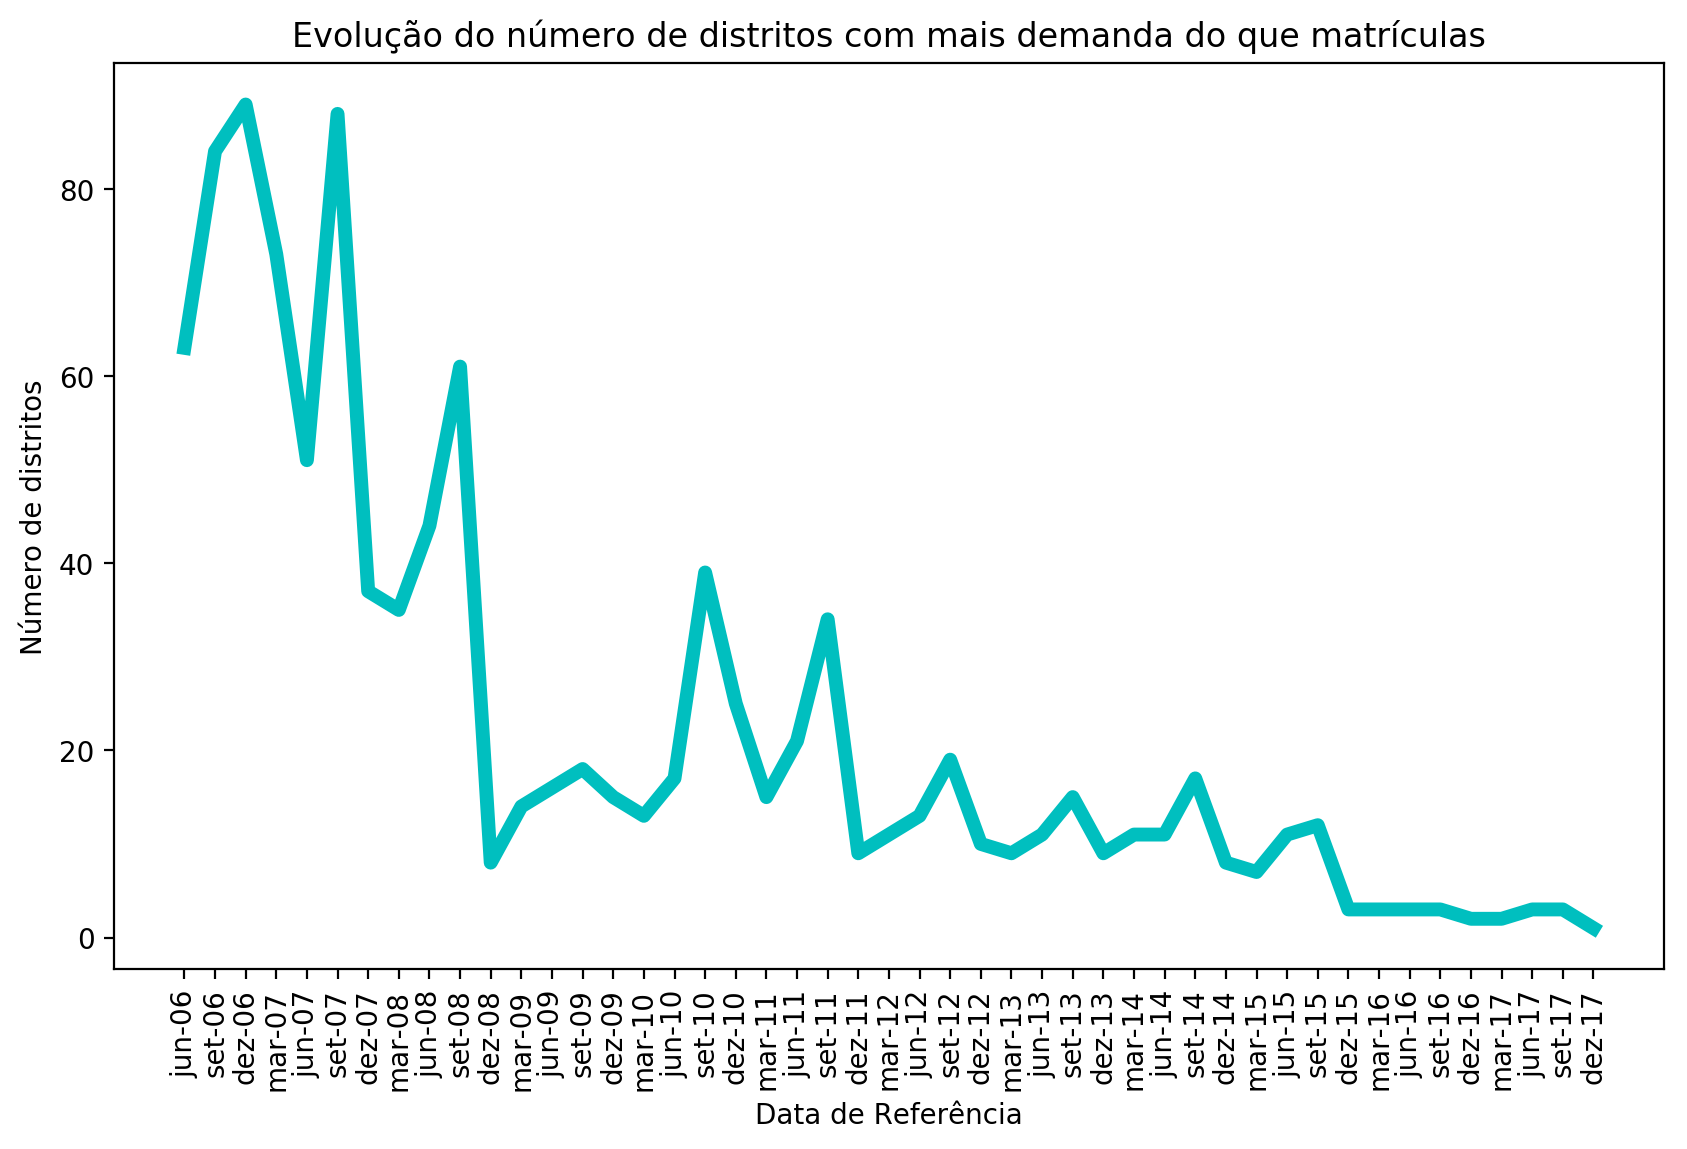
\includegraphics[width=.8\linewidth]{grafdem}
	\caption{Evolução do número de distritos com mais fila que matrículas.}
	\label{graf:dem}
\end{figure}

É curioso observar que esse número nunca chega a zero, nos períodos observados. O seu pico máximo foi atingido em dezembro de 2006, com 89 distritos nessa situação. 

Finalmente, destaque para alguns distritos. Para Marsilac, Jaguara e Lajeado, que atendem mais de 80\% da população estimada de 0 a 3 anos. Desses três, Lajeado tem o maior número de matrículas. No entanto, Marsilac pode ser considerado um \textit{outlier}, pois mesmo atendendo mais de 100\% da população considerada, ele tem a maior fila proporcional à população entre todos os distritos (26.6\%).

